\documentclass[UTF8]{ctexart}
\usepackage{boxedminipage}
\usepackage{float}
\usepackage{hyperref}
\usepackage{graphicx}
\usepackage{multirow}
\usepackage{array}
%================样式================
\usepackage[\VAR{geometry.header}]{geometry}
\setlength{\headsep}{\VAR{geometry.headsep}mm}
%\usepackage{setspace}
%\setstretch{1}
\usepackage{enumitem}
\setenumerate[1]{partopsep=0mm,parsep=\parskip,topsep=0mm}
%================交叉引用================
\renewcommand{\figureautorefname}{图}
%================快捷,与Python程序无关================
\newcommand{\smalltitle}[1]{{\zihao{4}\bfseries{#1}}\\} 
%================页眉================
\usepackage{fancyhdr}
\usepackage{lastpage}
\pagestyle{fancy}
\renewcommand{\headrulewidth}{0.5pt}
%\renewcommand{\footrulewidth}{0pt}
\fancyhf{}
\setlength{\headheight}{\VAR{geometry.headheight}mm}
\chead{
\centering
{\zihao{3}\textbf{生产作业指导书}}
}
%================正文的环境设置================
\begin{document}
\zihao{5}
\centering
%================正文内容================
\begin{boxedminipage}{\VAR{geometry.textwidth|round(2)}mm}
\centering
\smalltitle{开班准备描述}
\begin{boxedminipage}[t]{\VAR{intro_width|round(2)}mm}
\begin{enumerate}
\BLOCK{for i in 开班准备描述}
\item \VAR{i}
\BLOCK{endfor}
\end{enumerate}
\end{boxedminipage}
\hfill
\begin{boxedminipage}[t]{\VAR{picbox_width|round(2)}mm}
\begin{figure}[H]
\parbox[t]{\VAR{picbox_half_width|round(2)}mm}{
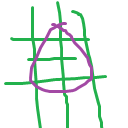
\includegraphics[width=\VAR{picbox_half_width|round(2)}mm]{pic01}
\caption{}}
\hfill
\parbox[t]{\VAR{picbox_half_width|round(2)}mm}{
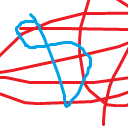
\includegraphics[width=\VAR{picbox_half_width|round(2)}mm]{pic02}
\caption{}}
\end{figure}
\end{boxedminipage}
\end{boxedminipage}

\begin{boxedminipage}{\VAR{geometry.textwidth|round(2)}mm}
\centering
\smalltitle{设备开机描述}
\begin{boxedminipage}[t]{\VAR{intro_width|round(2)}mm}
\begin{enumerate}
\BLOCK{for i in 设备开机描述}
\item \VAR{i}
\BLOCK{endfor}
\end{enumerate}
\end{boxedminipage}
\hfill
\begin{boxedminipage}[t]{\VAR{picbox_width|round(2)}mm}
图片2
\end{boxedminipage}
\end{boxedminipage}

\begin{boxedminipage}{\VAR{geometry.textwidth|round(2)}mm}
\centering
\setlength{\tabcolsep}{\VAR{check_table.tabcolsep}mm}
\smalltitle{检查项目}
\VAR{check_table.content}
\end{boxedminipage}
\end{document}